\documentclass[12pt]{article}

\usepackage{sbc-template}
\usepackage{graphicx,url}
\usepackage[utf8]{inputenc}
%\usepackage[brazil]{babel}
%\usepackage[latin1]{inputenc}  

     
\sloppy

\title{Guia para o uso do Geonode}

\author{NDS\inst{1}}


\address{
  NDS
\nextinstitute
  CPRM
\email{\{cprm,nds\}@sgb.gov.br}
}

\begin{document} 

\maketitle


\section{Introdução}

Este documento define procedimentos a serem utilizados para a carga de dados,
estilos e metadados no ambiente Geonode do Odisseia.

\section{Acesso} \label{sec:firstpage}

Para carregar arquivos no sistema Geonode, o usuário deve estar conectado em
uma conta com permissão para a carga. Para isso o usuário deve seguir o link na
parte superior direita da página para a tela de login e inserir suas
credenciais (Figura \ref{fig:login}).

\begin{figure}[h]
  \centering
  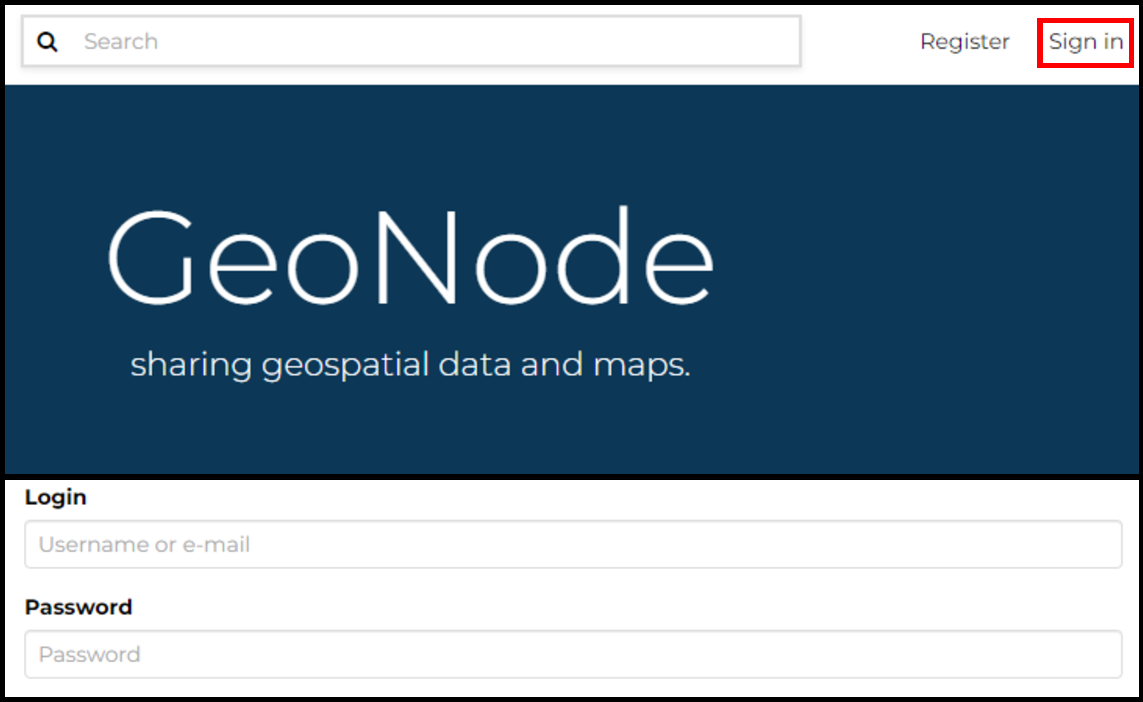
\includegraphics[width=\textwidth, keepaspectratio]{img/login.pdf}
  \caption{Caminho para a inserir as credenciais de login, em vermelho o link para acessar a página de login.}
  \label{fig:login}
\end{figure}


\section{Carga de Dados}

Com o acesso ao usuário com permissões para carga será possível visualizar o
menu de "Dados" no canto superior esquerda da página (Figura
\ref{fig:upload}.1). Duas opções estão disponíveis: datasets e documentos.
Datasets se referem aos arquivos de cunho de representação geoespacial
(shapefiles, geopackages, geojson, geotiff e outros) e documentos se referem
aos demais arquivos de registro de dados (pdf, jpeg, log, csv, zip e outros).

Após acessar o menu "Dados-Datasets" ou "Dados-Documentos" será possível
carregar novos dados utilizando o botão "Adicionar Recurso", no canto superior
direito da página (Figura \ref{fig:upload}.2). Em uma nova página o usuário
poderá utilizar o recurso de arrastar e soltar ou o botão de selecionar
arquivos no canto esquerdo da página (Figura \ref{fig:upload}.3), é possível
carregar mais de um arquivo durante este processo. Com os arquivos devidamente
selecionados o botão de "Upload" estará disponível para prosseguir o
carregamento (Figura \ref{fig:upload}.4). 

\textbf{Atenção, no caso de shapefiles será necessário que todos os seus
componentes sejam selecionados ou que todos os componentes sejam comprimidos em
um arquivo zip.}

Ao concluir o upload o usuário será redirecionado para uma página listando
todos os arquivos carregados. Ao clicar no nome do arquivo o usuário poderá
acessar sua página de detalhamento (Figura \ref{fig:upload}.5). O mesmo pode
ser feito através do menu "Dados" acessado anteriormente, clicando na imagem de
apresentação do dado e em seguida em visualizar.

Na página de detalhamento do dado é possível visualizar, filtrar e editar os
dados geoespaciais.

\begin{figure}[h]
  \centering
  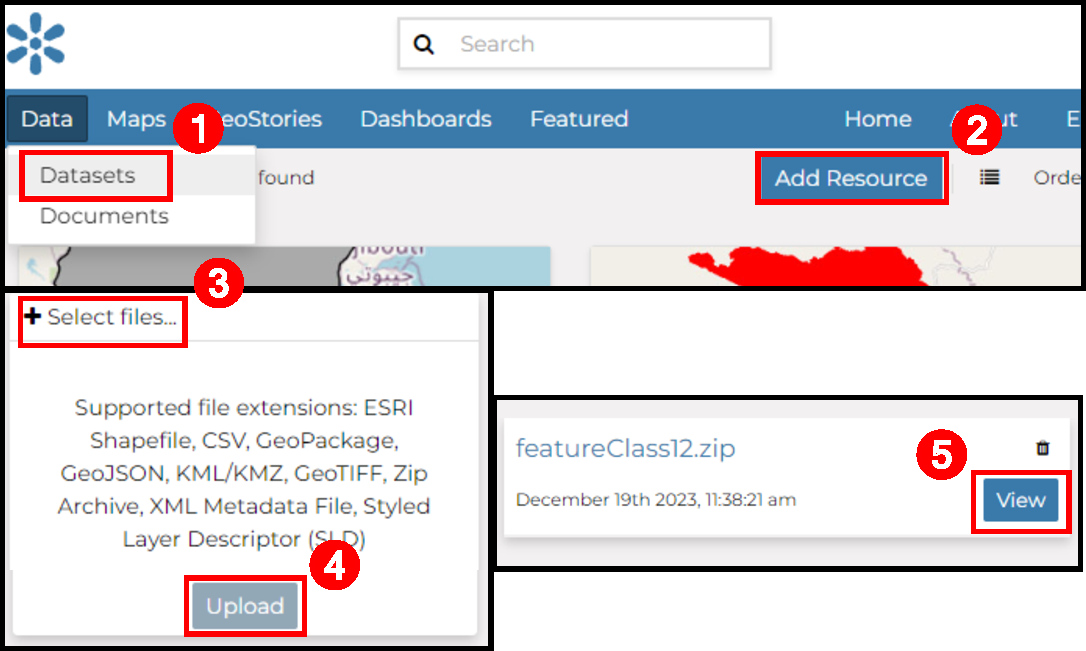
\includegraphics[width=\textwidth, keepaspectratio]{img/upload.pdf}
  \caption{Fluxo para o upload de dados no Geonode.}
  \label{fig:upload}
\end{figure}

\subsection{Estilo}

Na página de detalhamento de um dado é possível editar seu estilo através do
menu "Editar-Editar Estilo" (Figura \ref{fig:estilocodigo}.1).

O usuário pode utilizar o editor de estilo nativo do Geonode ou importar o
estilo do QGIS através de um arquivo SLD. Para importar estilos através do SLD
selecione o editor de código no canto superior direito do menu de edição de
estilo (Figura \ref{fig:estilocodigo}.2) e insira o texto de descrição SLD
criado pelo QGIS (Figura \ref{fig:estilocodigo}.3). Por fim aplique as
alterações (Figura \ref{fig:estilocodigo}.4).

\begin{figure}[h]
  \centering
  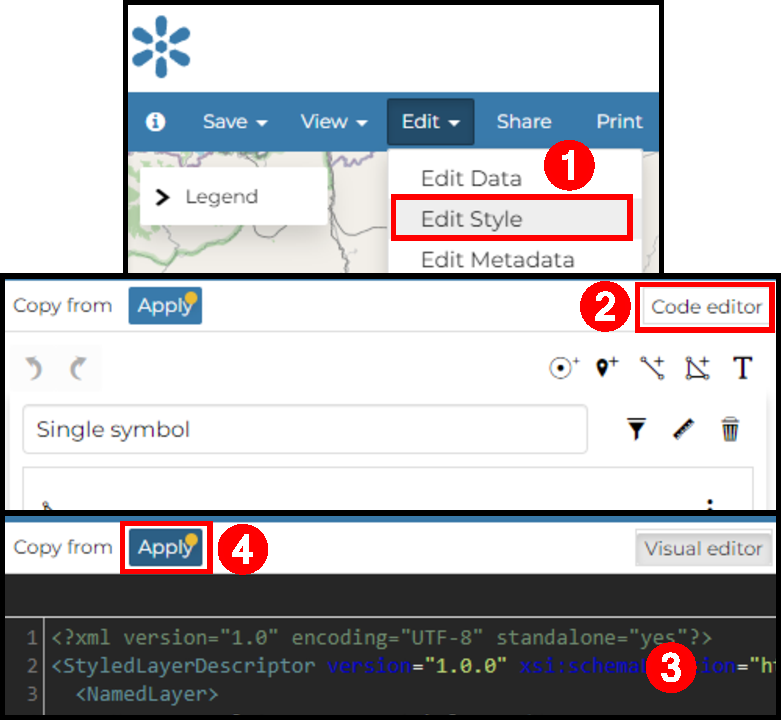
\includegraphics[width=\textwidth, keepaspectratio]{img/estilocodigo.pdf}
  \caption{Fluxo para a importação de estilo de um arquivo SLD.}
  \label{fig:estilocodigo}
\end{figure}

\subsubsection{Criando estilos SLD no QGIS}

No QGIS, na lista de camadas, clique com o botão direito na camada que deseja
exportar o estilo em SLD (Figura \ref{fig:exportarsld}.1). Siga para o menu
"Propriedades" e "Simbologia". No canto inferior esquerdo do menu simbologia
clique em "Estilo" e em seguida em "Salvar estilo" (Figura
\ref{fig:exportarsld}.2). No novo menu selecione o estilo SLD (Figura
\ref{fig:exportarsld}.3) e salve em um local a sua escolha.

\begin{figure}[h]
  \centering
  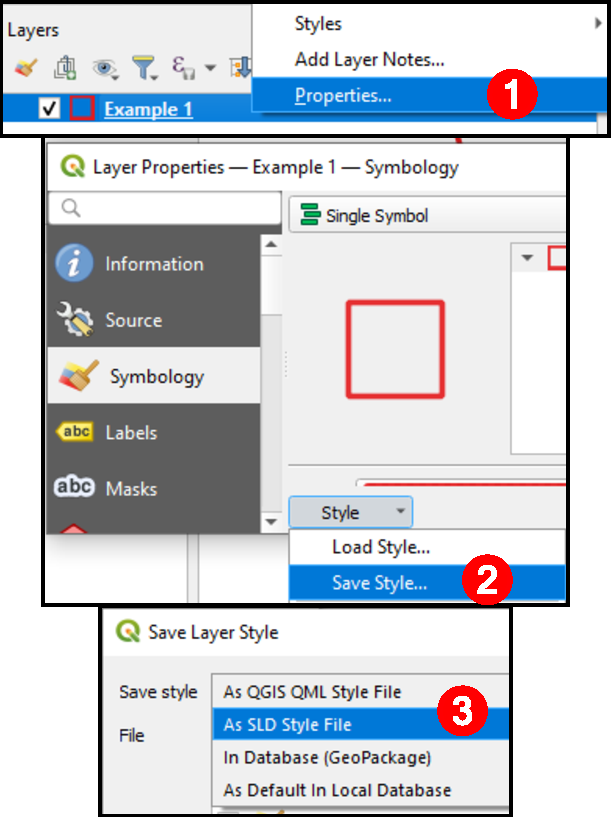
\includegraphics[keepaspectratio]{img/exportarsld.pdf}
  \caption{Fluxo para a exportação de um estilo para um arquivo SLD.}
  \label{fig:exportarsld}
\end{figure}

\subsection{Metadados}

Na página de detalhamento de um dado é possível editar seus metadados
através do menu "Editar-Editar Metadados".

Na página de edição de metadados o usuário pode alterar todos os aspectos do
metadado através de um formulário. A medida que os campos são completos uma
barra de progresso é atualizada. 

AQUI VAI UMA ESPECIFICAÇÃO SOBRE CADA METADADO?

\subsection{Mapas}

No menu Mapas na aba superior da página do Geonode é possível consultar os
mapas existentes e criar novos mapas. Usando o botão "Adicionar recursos" na
parte superior direita da página e em seguida "Criar mapa" é possível criar um
mapa a partir dos dados inseridos no Geonode.

\bibliographystyle{sbc}
\bibliography{sbc-template}

\end{document}
